% \documentclass[10pt, oneside, english]{article}   	
\documentclass[10pt, oneside]{article}
\usepackage{geometry}                		
\geometry{a4paper}                   		
% \usepackage[english, es-noindentfirst]{babel}
% \selectlanguage{english}
\usepackage[utf8]{inputenc}               		
\usepackage{graphicx}			
\usepackage{amssymb}
\usepackage{authblk}
\usepackage{multicol}
\usepackage{rotating}


\title{Word embeddings for predicting political affiliation based on Twitter data}

\author[]{Ibrahim Abdelaziz}
\author[]{Oliver Berg}
\author[]{Angjela Davitkova}
\author[]{Venkatesh Iyer}
\author[]{Shriram Selvakumar}
\author[]{Kumar Shridhar}
\author[]{Saurabh Varshneya}
\affil[1]{Technische Universität Kaiserslautern}

\date{\today}


\begin{document}
\maketitle
\begin{multicols}{2}


\section{Introduction}

The modern world of social media knows a plethora of means to communicate ones personal opinion and political alignment. With the platform \textit{Twitter}, figures of political interest are expressing their standpoints in small-sized 144 character texts (recently updated to 280 characters), which contain a comprised message specific to the general public. This yields great potential for automated analysis of party affiliations to classify political persons of interest within the overall political spectrum \cite{Biessmann2017}.

Hence, we propose a structured approach of building a deep learning based classification model that utilizes state-of-the-art \textbf{word embeddings} \cite{Pelevinala2016} to perform \textbf{qualitative analysis} on constructed \textbf{social media data set}. Our approach will be helpful in analyzing possible early intuitions and dedicated insights within the German political spectrum.

This is to be seen in context of latest \textbf{advances in research}.


\section{Related Work}

Political motives were shown to be consistently predictable with an accuracy better than chance \cite{Biessmann2017}.

Many existing papers either propose tackling the classification problem of political bias using techniques such as Support Vector Machine (SVM) or Singular Value Decomposition (SVD) \cite{Misra2016}, or they focus on comparison of different classifiers to not restrict themselves to a single well-developed approach \cite{Bhanda2009}. These approaches mainly consider the political affiliation in America, where the political orientation is mostly binary with two parties - republicans and democrats - covering most of the political spectrum.
Overall, sentiment classification is mostly covered using recurrent- or convolutional neural networks \cite{Kim2014}.

In connection to the given focus of working on Twitter data, \cite{Cohen2013} introduces objections to some of the pre-existing approaches. With standard classifiers for inferring political orientation having greatly lower accuracy compared to what was initially report, it is stated that the classifiers cannot be used for classifying users outside the training data. Thus the contradictory arguments hold true.


\section{Proposed Methodology}

As our approach aims to analyze text messages of political figures concerning party affiliation, we leverage \textit{word embeddings} to represent words in context. We shall initially restrict ourselves to a pre-trained model as the number of political parties as classes is not very high. A person's political affiliation will be calculated as a combined analysis of all of his Twitter messages.

Subsequently, a neural network architecture then classifies the Twitter profile, consisting of a collection of this person's tweets, concerning party affiliation. It will learn to represent a political figure's party affiliation through their expression in short message texts.

\subsection{Data Sets and Feature Extraction} 

The main portion of data collected will be Twitter data. In order to include all of the relevant politicians from the parties, their Twitter accounts with their corresponding messages will be collected, where the data is offered as open source data.
Each politicians own party is kept as his ground truth class label.

In order to train models on text, the data needs to be converted into numerical values, more specifically vectors, under specific similarity metrics. One way this can be achieved is to create a word embedding for each of the words from the tweets using \textit{Word2Vec} \cite{DBLP:journals/corr/abs-1301-3781}. While constructing word embeddings, appropriate dimensionality reduction can be applied.

There are seven class labels as there are seven political parties to consider, namely "CDU", "CSU", SPD", "FDP", "GRÜNE", "LINKE" and "AFD", ordered by age of introduction into German parliament, old to new. As such, a pre-trained word embeddings model should suffice to represent textual influence in regard to this relatively small number of classes.
Alternatively, a custom model may be trained on Wikipedia data dump in German language, possibly in combination with more politically motivated data sources such as German parliament discussion data or party manifesto data. 

For each party, the same number of accounts and tweets per account will be used to later train the classification model.

Train-test-splits with ration 80-20 will be employed, where the collection of a single person's tweets will be counted as a single data record. It may not be humanly feasible to classify a person's party affiliation based on a single Twitter message, and as such this should also not be the classifier's primary objective.

To recap, we propose to accumulate twitter-data per political figure and treat this collection as singular data records. Each record is associated with a single class label, depicting his truely associated party. Records are represented in numerical format by applying word embedding techniques. 

\subsection{Classification}

We propose a solution that will leverage neural networks, where we expect to compare both convolutional- and recurrent network architectures for the classification task.

We first aim to learn information of single words through a convolutional neural network (CNN) architecture. This has been proven to yield respectable results \cite{Kim2014}.

Formally, our training data would be textual information as described above from different users, encoded in form of word-embeddings. We combine randomly 'n' tweet embeddings of one user and assign it the label as one of the seven parties to which it belongs. The labels will be encoded in the form of one hot vectors. Loss can be computed in such case of multi-class scenario as the cross-entropy loss, defined as:
\begin{equation}
%x =y+z
H_{y'}(y) = - \sum_{i} y'_{i} \log (y_{i})
\end{equation}
Where \(y\) is our predicted probability distribution, and \(y'\) is the true distribution (the one-hot vector with the true-class party labels) 

Intuitively though, using a Long Short Term Memory (LSTM) recurrent neural network (RNN) architecture also seems like a good solution for the task at hand. It may smoothly correlate given words with their predecessors to not only take fixed content length into account like feed-forward networks do \cite{Sundermeyer2012lstm}.

Since the twitter dataset is very complex - given its small length and condense information characteristics - a default recurrent neural network alone may not be able to learn the most important features.


\section{Quantitative Analysis}

For a final quantitative analysis of the preceding findings, we propose statistical metrics such as Pearson Correlation Coefficient \cite{Hauke2011}, F1-Score and Cosine Similarities for the classification results.

Dataset visualization techniques like T-SNE \cite{Laurens2008} and PCA \cite{Richardson2009} will be utilized to display the overall positioning of the political entities.Further, we will experiment with new embedding techniques for visualizing semantic and syntactic analogies, described in \cite{8019864}, and the corresponding tests to determine whether the resulting views capture salient structures like words used by a specific party, specific accent used and more. Also, we will motivate clustering to find interesting single entities which are e.g. analyzed to not affiliate themselves with their original political party but another group of individuals, possibly from multiple different parties.

An experimental approach, which will be assessed but possibly not fully implemented will be to apply regression in addition to earlier classification to position political entities on a political scale like displayed in the "political compass" \cite{PoliticalCompass2017}. This could also take discussion and messaging between parties into account.
However, due to the different characteristics of this task compared to the earlier proposed classification task, this shall be done on a more exploratory basis. 

The overall goal of the quantitative analysis will be to find distinct characteristics of interest within a political figure's textual expression. As such, we aim to identify e.g. quality of language, usage of posh and / or infrequently used expressions or occurrence of accented language.
Being able to statistically correlate factual, emotional or radical language features to political identities and organizations would conclude our findings.


\end{multicols}
\newpage

\section{Appendix - Work packages and distribution}

We plan to distribute the workload into the work packages, for each work package we assign a group of people, and an initial estimated deadline.

\begin{flushleft}
\textbf{Building dataset}

Beside the Tweets of German politicians that we will get using the Twitter API, we also plan to collect data from other sources such as parliament discussion data and party manifesto data.
\end{flushleft}

\begin{flushleft}
\textbf{Training word vector model}

After building our dataset we will convert the data text into numerically creating word embedding of the words in the text using Word2Vec or derived approaches.
\end{flushleft}

\begin{flushleft}
\textbf{Developing classification model}

As previously mentioned in the Proposed Methodology we will implement a neural network as our classifier, and train it with our data set.
\end{flushleft}

\begin{flushleft}
\textbf{Training / Testing}

After having quantified model accuracy with a dedicated validation split, this separate training- and testing-stage ensures that the obtained results match initial expectations or reject estimates in an understandable fashion. We thereby ensure that the obtained results obey logic and real-world measures.
\end{flushleft}

\begin{flushleft}
\textbf{Quantitative Analysis}

To conclude the findings from real-word social media data analysis, we infer statistical and sociological meaning to the modeled results and put them in context to the initially motivated research question of political affiliation and political classification.
\end{flushleft}

\begin{sidewaysfigure}
  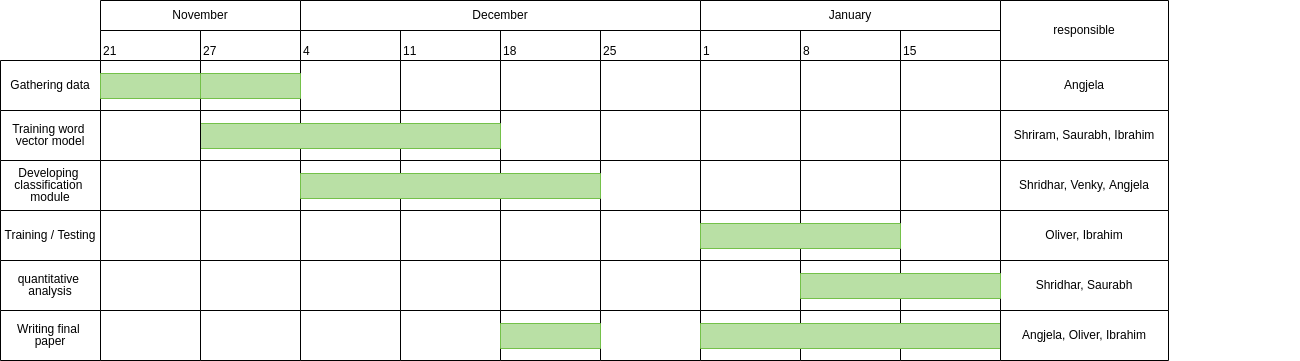
\includegraphics[width=\textwidth]{gantt.png}
  \caption{Gantt-Chart displaying workload distribution per team-member}
\end{sidewaysfigure}


\bibliography{lit}
\bibliographystyle{apalike}

\end{document} 
